\chapter{Resposta às Perguntas}

\section{O que é o anel de chaves privadas?}
O anel de chaves privadas (private keyring) é uma estrutura de dados que armazena as chaves privadas do usuário no sistema PGP/GPG. Diferente do anel de chaves públicas, esse repositório contém material criptográfico altamente sensível que deve ser protegido \cite{gnupgprivate}.

\subsection{Estrutura do anel de chaves privadas}
\begin{itemize}
    \item Cada entrada no anel de chaves contém uma chave privada principal e possivelmente várias subchaves.
    \item Cada chave privada armazenada inclui:
    \begin{itemize}
        \item A chave privada em si (material criptográfico para decriptação/assinatura)
        \item Identificadores de usuário associados (nome, email, comentário)
        \item Data de criação e expiração
        \item Flags de uso (assinatura, criptografia, autenticação)
        \item Informações de preferências criptográficas
        \item O material criptográfico é armazenado de forma protegida, geralmente usando criptografia simétrica com uma senha como chave.
    \end{itemize}
\end{itemize}

\subsection{Localização do armazenamento no GnuPG}
\begin{itemize}
    \item Nas versões modernas do GnuPG (2.1+), o anel de chaves privadas é armazenado no diretório \texttt{\~{}/.gnupg/private-keys-v1.d/} como arquivos individuais para cada chave \cite{gnupgprivate}.
    \item Em versões mais antigas (GnuPG 1.x), as chaves privadas eram armazenadas em um único arquivo chamado \texttt{secring.gpg} no diretório \texttt{\~{}/.gnupg/} \cite{gnupgdoc}.
    \item No macOS (que foi usado neste trabalho), esse diretório está localizado em \texttt{/Users/joaopedroschmidtcordeiro/.gnupg/}.
\end{itemize}

\begin{figure}[htb]
    \centering
    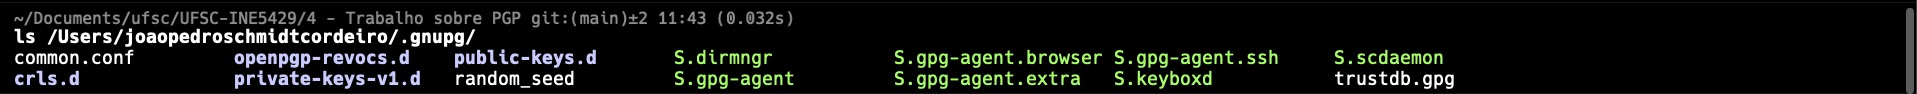
\includegraphics[width=0.8\textwidth]{images/04-anel_chaves_privadas.jpg}
    \caption{Anel de chaves privadas}
    \label{fig:anel-chaves-privadas}
\end{figure}

\subsection{Proteção e acesso}
\begin{itemize}
    \item O acesso ao anel de chaves privadas é restrito apenas ao proprietário da chave.
    \item A proteção ocorre em dois níveis:
    \begin{enumerate}
        \item \textbf{Proteção no sistema de arquivos}: O diretório e os arquivos têm permissões restritas (geralmente 600 ou 700, que permitem acesso somente ao proprietário).
        \item \textbf{Proteção criptográfica}: Cada chave privada é criptografada com uma senha definida pelo usuário. Essa senha é necessária para qualquer operação que utilize a chave privada.
    \end{enumerate}
    \item Apenas o proprietário do diretório \texttt{\~{}/.gnupg/} pode acessar os arquivos de chave privada, desde que mantenha as permissões de arquivo adequadas.
    \item Mesmo tendo acesso aos arquivos, um atacante ainda precisaria da senha para usar as chaves privadas.
    \item O GPG Agent gerencia o cache temporário de senhas, permitindo que operações subsequentes sejam realizadas sem digitar a senha repetidamente dentro de um período configurável.
\end{itemize}

\begin{figure}[htb]
    \centering
    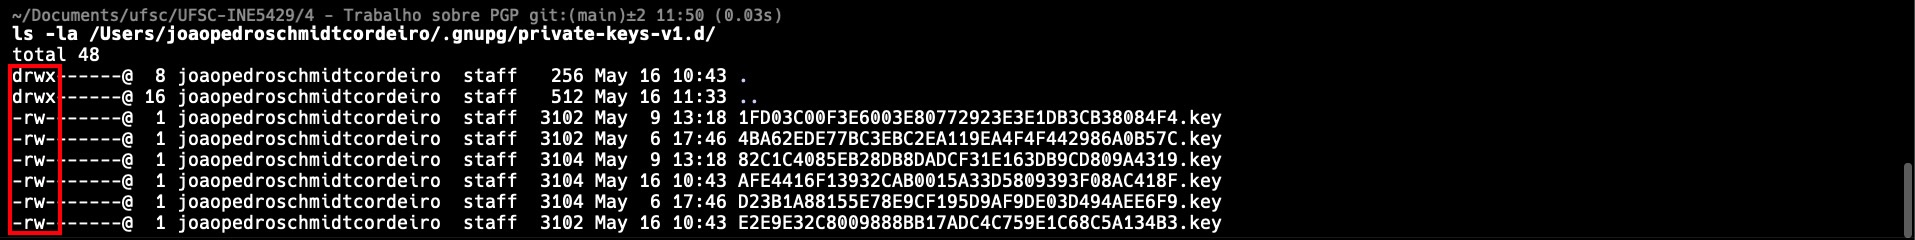
\includegraphics[width=0.8\textwidth]{images/04-permissoes_anel_chaves_privadas.jpeg}
    \caption{Permissões do anel de chaves privadas}
    \label{fig:permissoes-anel}
\end{figure}

Por essas razões, é crucial manter a segurança do sistema operacional, usar senhas fortes para proteger as chaves privadas e considerar o uso de hardware tokens (como YubiKey) para armazenar as chaves privadas em dispositivos físicos separados para maior segurança \cite{pgpbest}.

\section{Qual a diferença entre assinar uma chave local e assinar no servidor?}

\subsection{Assinatura local (não exportada)}
\begin{itemize}
    \item A assinatura é armazenada apenas no chaveiro local do signatário
    \item É criada usando o comando \texttt{gpg --lsign-key ID\_DA\_CHAVE} ou usando a opção de assinatura local no modo interativo
    \item Não é enviada automaticamente para servidores de chaves públicos
    \item É visível apenas para o signatário e qualquer pessoa com acesso ao seu chaveiro local
    \item Útil para validar chaves para uso pessoal sem fazer uma declaração pública de confiança
    \item Não contribui para a Web of Trust global do PGP \cite{gnupgsig}
\end{itemize}

\subsection{Assinatura em servidor (exportada/pública)}
\begin{itemize}
    \item A assinatura é criada localmente e depois enviada a servidores de chaves públicos
    \item É criada usando \texttt{gpg --sign-key ID\_DA\_CHAVE} e depois enviada com \texttt{gpg --send-key ID\_DA\_CHAVE}
    \item Torna-se disponível publicamente para qualquer pessoa que consulte a chave nos servidores
    \item Serve como uma declaração pública de que você verificou a identidade do proprietário da chave
    \item Contribui para a Web of Trust do PGP, ajudando outras pessoas a avaliar a autenticidade da chave
    \item Tem implicações de privacidade, pois revela sua associação com o proprietário da chave
\end{itemize}

A principal diferença está na visibilidade e no propósito. Assinaturas locais são privadas e para uso pessoal, enquanto assinaturas em servidor são públicas e contribuem para estabelecer a credibilidade da chave na comunidade PGP global. Além disso, uma vez publicada em servidores, uma assinatura é praticamente impossível de ser completamente removida, devido à natureza distribuída dos servidores de chaves PGP \cite{gnupgkeysigning}.

No caso dos experimentos realizados neste trabalho, foram utilizadas assinaturas públicas que foram enviadas ao servidor, como demonstrado nas capturas de tela anteriores. Isso permitiu que a assinatura fosse verificada publicamente e, posteriormente, também permitiu demonstrar o processo de revogação da assinatura.

\section{O que é e como é organizado o banco de dados de confiabilidade?}

O banco de dados de confiabilidade (trustdb) no PGP é uma estrutura que armazena informações sobre o quanto você confia nas chaves públicas e nas pessoas que assinaram essas chaves. Este banco de dados é uma parte fundamental do modelo de confiança descentralizado do PGP, conhecido como "Web of Trust" (Teia de Confiança) \cite{gnupgwot}.

\subsection{Definição e função}
\begin{itemize}
    \item O trustdb é um arquivo que armazena metadados sobre a confiança que você atribui às chaves em seu chaveiro
    \item Ele não contém as chaves em si, apenas as relações de confiança entre elas
    \item Seu propósito é permitir ao GnuPG calcular automaticamente a validade das chaves usando o modelo de confiança do PGP
\end{itemize}

\subsection{Localização e formato}
\begin{itemize}
    \item No GnuPG, o banco de dados de confiabilidade é armazenado no arquivo \texttt{\~{}/.gnupg/trustdb.gpg}
    \item É um arquivo binário, não destinado a ser editado diretamente
    \item É local para cada usuário, ou seja, seu banco de confiabilidade reflete apenas suas próprias relações de confiança
\end{itemize}

\subsection{Níveis de confiança}
O GnuPG utiliza vários níveis de confiança para as chaves:

\subsubsection{Validade da chave}
\begin{itemize}
    \item Desconhecida: Não há informações suficientes para determinar a validade
    \item Inválida: A chave é considerada inválida por algum motivo
    \item Marginalmente válida: A chave tem alguma validade, mas não o suficiente para confiança total
    \item Completamente válida: A chave é considerada autêntica
\end{itemize}

\subsubsection{Confiança no proprietário (owner-trust)}
\begin{itemize}
    \item Indefinida (não definida): Nenhum nível de confiança foi atribuído
    \item Nunca confiar: Você não confia no proprietário para assinar outras chaves
    \item Confiança marginal: Você confia parcialmente no proprietário para assinar outras chaves
    \item Confiança total: Você confia plenamente no proprietário para assinar outras chaves
    \item Confiança definitiva: Reservado para suas próprias chaves
\end{itemize}

\subsection{Organização e cálculo da validade}
O GnuPG usa um algoritmo para calcular a validade das chaves baseado no seguinte \cite{gnupgwot}:

\begin{itemize}
    \item Uma chave é completamente válida se você assinou diretamente (confiança definitiva)
    \item Uma chave pode se tornar válida se for assinada por um número suficiente de pessoas em quem você confia:
    \begin{itemize}
        \item Uma assinatura de alguém com confiança total
        \item Várias assinaturas (geralmente 3) de pessoas com confiança marginal
    \end{itemize}
    \item Este sistema permite que a confiança se propague através da rede (Web of Trust)
\end{itemize}

\subsection{Visualização e gerenciamento}
Você pode visualizar e gerenciar o banco de dados de confiabilidade usando os seguintes comandos:

\begin{lstlisting}[language=bash]
# Visualizar os níveis de confiança atuais
gpg --list-keys --with-colons

# Editar a confiança de uma chave
gpg --edit-key ID_DA_CHAVE
> trust
> (selecione o nível de confiança)
> save

# Verificar a integridade do banco de dados de confiabilidade
gpg --check-trustdb
\end{lstlisting}

O banco de dados de confiabilidade é pessoal e reflete suas próprias decisões sobre em quem confiar. Não é enviado aos servidores de chaves e permanece privado em seu sistema. Isso permite que cada usuário do PGP construa sua própria rede de confiança, baseada em suas interações pessoais e verificações de identidade \cite{pgpbest} \cite{gnupgwot}.

\section{O que são e para que servem as sub-chaves?}

As subchaves no PGP são chaves criptográficas secundárias associadas a uma chave primária (ou mestra) que funcionam como componentes especializados dentro do mesmo certificado PGP. Enquanto a chave primária estabelece sua identidade digital, as subchaves são utilizadas para operações específicas do dia-a-dia \cite{gnupgdoc}.

\subsection{Definição e estrutura}
\begin{itemize}
    \item Uma subchave é uma chave criptográfica adicional que está vinculada criptograficamente à chave primária
    \item Cada subchave pode ter sua própria data de expiração, tamanho e algoritmo
    \item As subchaves são assinadas pela chave primária, estabelecendo uma relação de confiança e autenticidade
    \item Um certificado PGP moderno geralmente contém uma chave primária e várias subchaves especializadas
\end{itemize}

\subsection{Tipos de subchaves}
\begin{enumerate}
    \item \textbf{Subchave de assinatura (S)}: Usada para assinar mensagens, arquivos e outras chaves
    \item \textbf{Subchave de criptografia (E)}: Usada exclusivamente para criptografar dados
    \item \textbf{Subchave de autenticação (A)}: Usada para autenticação em sistemas (como SSH)
\end{enumerate}

\subsection{Propósitos e vantagens}
\begin{itemize}
    \item \textbf{Segurança aprimorada}: A chave primária pode ser mantida offline em local seguro, enquanto as subchaves são usadas no dia a dia
    \item \textbf{Revogação seletiva}: Se uma subchave for comprometida, ela pode ser revogada sem afetar a chave primária ou outras subchaves
    \item \textbf{Separação de funções}: Diferentes subchaves podem ser utilizadas para diferentes dispositivos ou contextos
    \item \textbf{Renovação flexível}: As subchaves podem ter períodos de validade mais curtos e serem renovadas sem afetar a identidade principal
    \item \textbf{Redução da exposição}: A chave primária é usada apenas para certificação (assinatura de subchaves e IDs de usuário), limitando sua exposição a riscos
\end{itemize}

\subsection{Funcionamento prático}
Quando você usa PGP no dia a dia, na realidade está utilizando suas subchaves para a maioria das operações. Por exemplo:
\begin{itemize}
    \item Ao assinar um documento: sua subchave de assinatura é utilizada
    \item Ao receber uma mensagem criptografada: sua subchave de criptografia é usada para decifrar
    \item Ao autenticar-se em um servidor via SSH-GPG: sua subchave de autenticação é empregada
\end{itemize}

\subsection{Gerenciamento}
\begin{lstlisting}[language=bash]
# Listar chaves com subchaves
gpg --list-keys --with-subkey-fingerprints

# Adicionar uma nova subchave
gpg --edit-key SEU_ID_DE_CHAVE
> addkey
> (selecionar tipo, tamanho, expiração)
> save

# Revogar uma subchave
gpg --edit-key SEU_ID_DE_CHAVE
> key N (selecionar número da subchave)
> revkey
> save
\end{lstlisting}

Esse design com subchaves é uma característica fundamental que diferencia o OpenPGP de outros sistemas de criptografia de chave pública, proporcionando um equilíbrio entre segurança e usabilidade. O modelo permite que você mantenha sua identidade digital (chave primária) altamente protegida, enquanto utiliza ferramentas mais expostas (subchaves) para operações cotidianas \cite{gnupgprivate}.

\section{Coloque sua foto (ou uma figura qualquer) que represente você em seu certificado PGP}

Os certificados PGP permitem adicionar uma foto ou imagem como elemento de identificação visual, o que proporciona uma camada adicional de verificação de identidade quando outras pessoas usam sua chave \cite{gnupgdoc}. Para adicionar uma foto ao certificado PGP, foram seguidos os passos abaixo:

\subsection{Preparação da imagem}
\begin{itemize}
    \item Foi selecionada uma imagem representativa em formato JPEG
    \item A imagem foi redimensionada para um tamanho apropriado (recomendado menor que 240x288 pixels)
    \item A imagem foi salva como \texttt{foto\_perfil.jpg} no diretório do projeto
\end{itemize}

\subsection{Processo de adição da foto}
\begin{lstlisting}[language=bash]
# Entrando no modo de edição da chave principal
gpg --edit-key 5BD7096F81478AA33F6CB0B4155B13B98FE2E6C8

# No prompt interativo, uso do comando addphoto
> addphoto

# Informação do caminho para o arquivo de imagem
> ./foto_perfil.jpg

# Confirmação da adição da foto
> y

# Salvando as alterações
> save
\end{lstlisting}

\begin{figure}[htb]
    \centering
    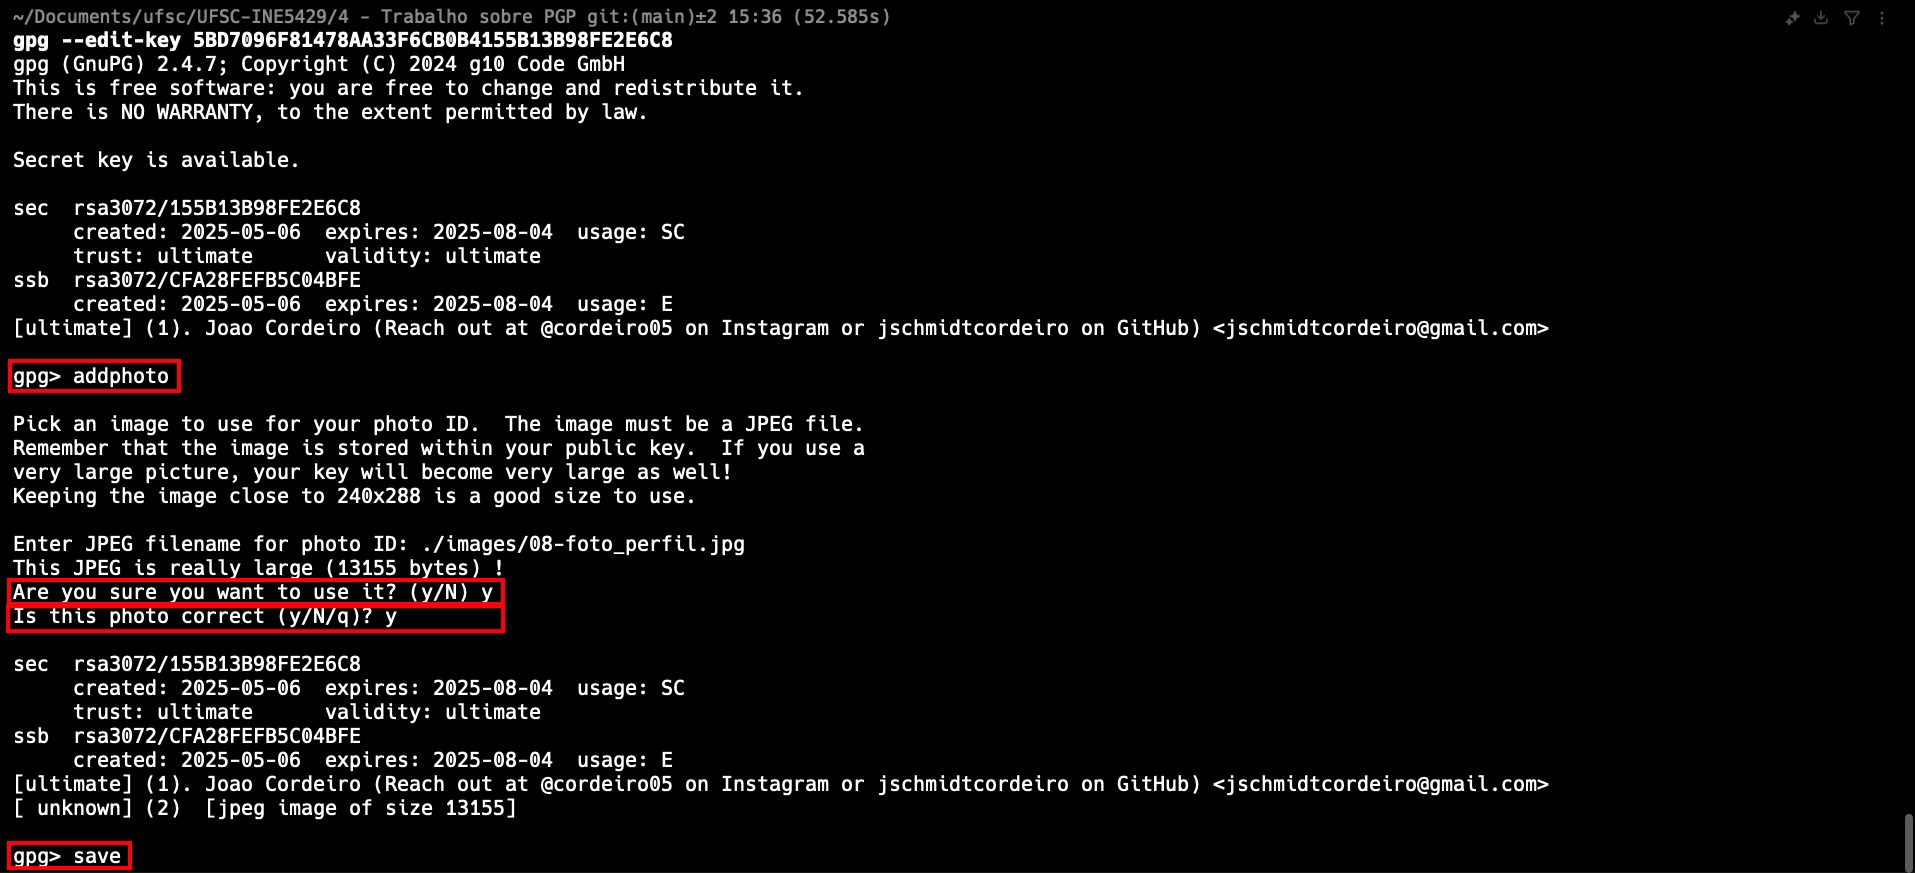
\includegraphics[width=0.8\textwidth]{images/08-adicao_foto_certificado.jpeg}
    \caption{Adição da foto ao certificado}
    \label{fig:adicao-foto}
\end{figure}

\subsection{Verificação da foto no certificado}
Para confirmar que a foto foi adicionada corretamente ao certificado, foi executado:

\begin{lstlisting}[language=bash]
# Verificação da foto no certificado
gpg --edit-key 5BD7096F81478AA33F6CB0B4155B13B98FE2E6C8
> showphoto
> quit
\end{lstlisting}

\begin{figure}[htb]
    \centering
    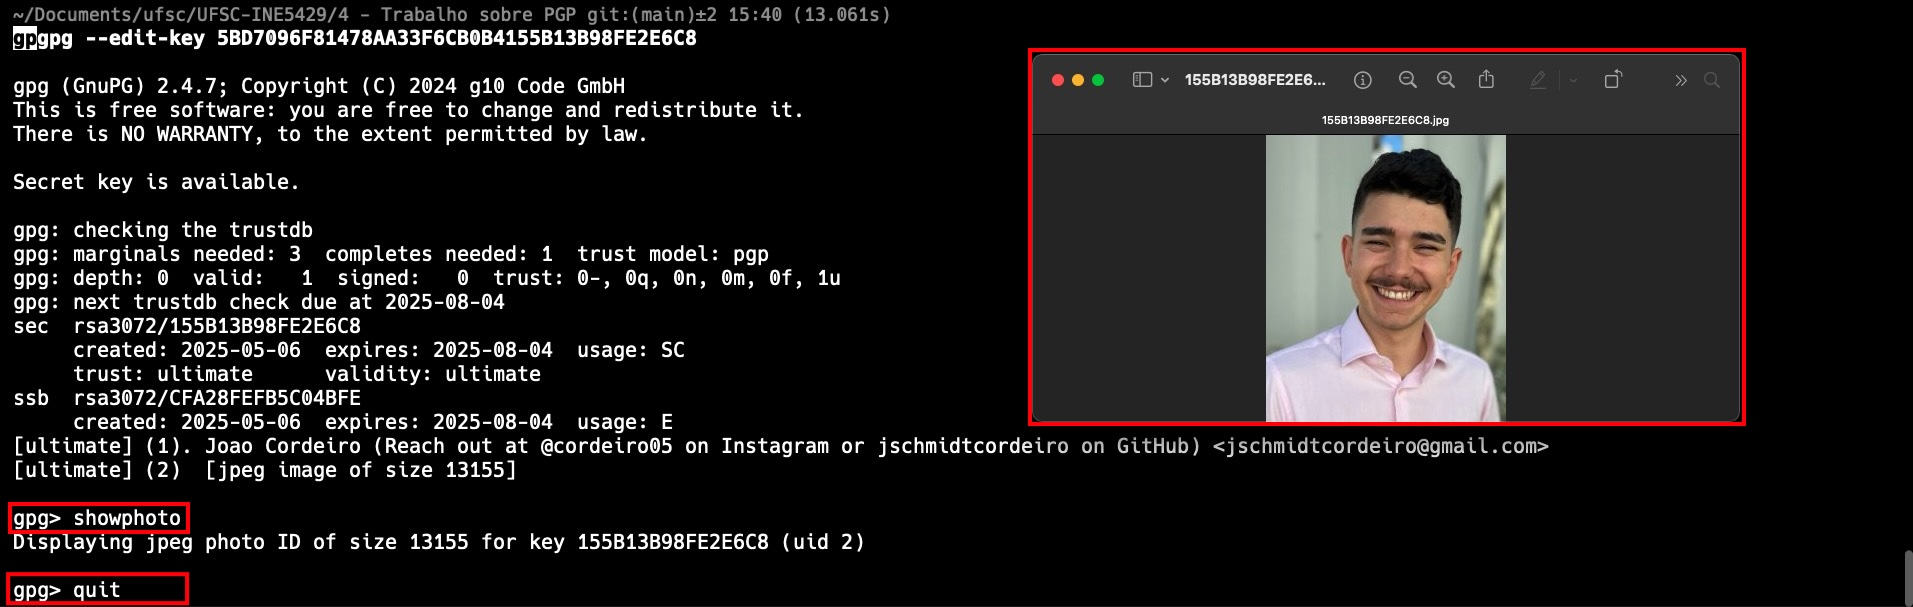
\includegraphics[width=0.8\textwidth]{images/08-verificacao_foto_certificado.jpeg}
    \caption{Verificação da foto no certificado}
    \label{fig:verificacao-foto}
\end{figure}

\subsection{Observações sobre segurança}
Adicionar uma foto ao certificado aumenta ligeiramente o tamanho da chave pública e oferece um método visual para confirmar a identidade do proprietário da chave. No entanto, isso também reduz o anonimato, já que qualquer pessoa que tenha acesso à chave pública também terá acesso à imagem. Por isso, é importante escolher uma imagem apropriada e considerar as implicações de privacidade \cite{pgpbest}.

\subsection{Atualização do servidor de chaves}
Após adicionar a foto, a chave atualizada foi enviada para o servidor:

\begin{lstlisting}[language=bash]
# Enviando a chave atualizada para o servidor
gpg --keyserver keyserver.ubuntu.com --send-key 5BD7096F81478AA33F6CB0B4155B13B98FE2E6C8
\end{lstlisting}

\begin{figure}[htb]
    \centering
    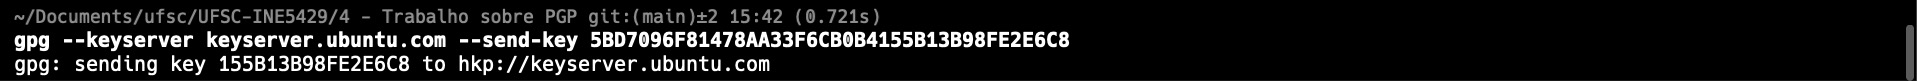
\includegraphics[width=0.8\textwidth]{images/08-envio_chave_atualizada.jpg}
    \caption{Envio da chave atualizada}
    \label{fig:envio-chave-atualizada}
\end{figure}

\section{O que é preciso para criar e manter um servidor de chaves PGP sincronizado com os demais servidores existentes?}

Criar e manter um servidor de chaves PGP sincronizado com a rede global de servidores envolve diversos componentes técnicos, configurações de rede e considerações de infraestrutura \cite{koch2018keyserver}. Os servidores de chaves são fundamentais para a infraestrutura de chave pública do OpenPGP, permitindo que os usuários publiquem, descubram e obtenham chaves públicas.

\subsection{Requisitos de hardware}
\begin{itemize}
    \item Servidor dedicado ou máquina virtual com recursos adequados \cite{sksdoc}:
    \begin{itemize}
        \item CPU: 2-4 núcleos (mais para servidores de alto tráfego)
        \item RAM: 4-8 GB mínimo (mais para bancos de dados grandes)
        \item Armazenamento: 20-50 GB mínimo, preferencialmente SSD para melhor desempenho
        \item Conexão de rede estável e rápida com endereço IP fixo
        \item Largura de banda suficiente para lidar com tráfego e sincronização
    \end{itemize}
\end{itemize}

\subsection{Software e configuração}
\begin{itemize}
    \item Sistema operacional: Linux (como Debian, Ubuntu Server ou CentOS)
    \item Software de servidor de chaves (existem algumas opções) \cite{fiskerstrand2019guide}:
    \begin{itemize}
        \item SKS (Synchronizing Key Server) - tradicional, mas com limitações de manutenção
        \item Hagrid - mais moderno, usado por keys.openpgp.org
        \item OpenPGP CA - para ambientes corporativos
        \item pgp-keyserver-lite - implementação mais leve
    \end{itemize}
    \item Configuração de DNS com registros A e PTR corretamente configurados
    \item Certificados TLS/SSL para comunicação segura (HTTPS)
    \item Servidor web como Nginx ou Apache para proxy reverso
\end{itemize}

\subsection{Processo de sincronização}
\begin{enumerate}
    \item \textbf{Membership}: Configurar o servidor para participar da rede SKS ou equivalente \cite{sksdoc}
    \item \textbf{Peering}: Estabelecer conexões com outros servidores de chaves (peers)
    \item \textbf{Reconciliação}: Processo pelo qual os servidores trocam informações sobre as chaves que possuem
    \item \textbf{Recon}: Transferência efetiva de chaves faltantes entre servidores
    \item \textbf{Programação de sincronização}: Configurar intervalos regulares para sincronização
\end{enumerate}

\subsection{Considerações de segurança}
\begin{itemize}
    \item Firewall corretamente configurado para permitir apenas tráfego necessário
    \item Monitoramento de segurança e registro de eventos
    \item Atualizações regulares de segurança para todos os componentes
    \item Proteção contra ataques DDoS
    \item Implementação de mitigações para problemas como "certificate spamming" \cite{hansen2019poisoning}
\end{itemize}

\subsection{Desafios e problemas conhecidos}
\begin{itemize}
    \item \textbf{Spam de certificados}: Chaves podem ser "poluídas" com muitas assinaturas \cite{hansen2019poisoning}
    \item \textbf{Remoção impossível}: Pela natureza descentralizada, chaves são difíceis de remover completamente
    \item \textbf{Requisitos de armazenamento crescentes}: O banco de dados apenas cresce
    \item \textbf{Problemas de privacidade}: Servidores tradicionais expõem todos os detalhes das chaves
    \item \textbf{Manutenção do SKS}: O software tradicional SKS não é mais ativamente mantido \cite{sksdoc}
\end{itemize}

\subsection{Abordagens modernas}
\begin{itemize}
    \item Servidores como keys.openpgp.org implementam verificação de e-mail \cite{keysopenpgp}
    \item Algumas implementações modernas permitem remoção de informações pessoais
    \item Os novos servidores podem optar por filtrar metadados sensíveis
    \item Rede federada com políticas consensuais entre operadores
\end{itemize}

\subsection{Passos para implementação}
\begin{enumerate}
    \item Preparar infraestrutura e instalar sistema operacional
    \item Instalar e configurar o software do servidor de chaves \cite{koch2018keyserver}
    \item Configurar sincronização com outros servidores
    \item Configurar certificados TLS/SSL e servidor web
    \item Estabelecer políticas de backup e recuperação
    \item Configurar monitoramento e alertas
    \item Documentar procedimentos operacionais
    \item Inscrever-se em listas de discussão relevantes para manter-se atualizado sobre mudanças nos protocolos
\end{enumerate}

A manutenção de um servidor de chaves PGP requer compromisso contínuo, atualizações regulares e monitoramento para garantir que ele continue sendo um recurso confiável e seguro para a comunidade PGP \cite{fiskerstrand2019guide}.

\section{Dê um exemplo de como tornar sigiloso um arquivo usando o PGP}

Para demonstrar o processo de tornar um arquivo sigiloso usando o PGP, foi realizado um experimento de troca de arquivos criptografados com um colega César Augusto. A comunicação foi feita de forma assíncrona, com cada um criptografando e enviando um arquivo, seguido pela decriptografia do arquivo recebido.

\subsection{Parte 1: Criptografando e enviando um arquivo sigiloso}

\subsubsection{Preparação do arquivo para envio}
\begin{itemize}
    \item Foi criado um arquivo de texto com informações sensíveis chamado \texttt{mensagem\_secreta.txt}
    \item O arquivo continha uma mensagem pessoal que deveria ser lida apenas pelo destinatário
\end{itemize}

\begin{lstlisting}[language=bash]
# Criação do arquivo de exemplo
echo "Esta é uma mensagem secreta para o César Augusto. Só ele deve conseguir ler!" > mensagem_secreta.txt
\end{lstlisting}

\subsubsection{Obtenção da chave pública do destinatário}
Para criptografar o arquivo, foi necessário usar a chave pública do destinatário. Como a chave do César Augusto já havia sido importada em experimentos anteriores, sua presença no chaveiro foi verificada:

\begin{lstlisting}[language=bash]
# Verificação da chave do César Augusto no chaveiro
gpg --list-keys 83501B6CED80BF3E2473308E9915F44F5835C85C
\end{lstlisting}

\begin{figure}[htb]
    \centering
    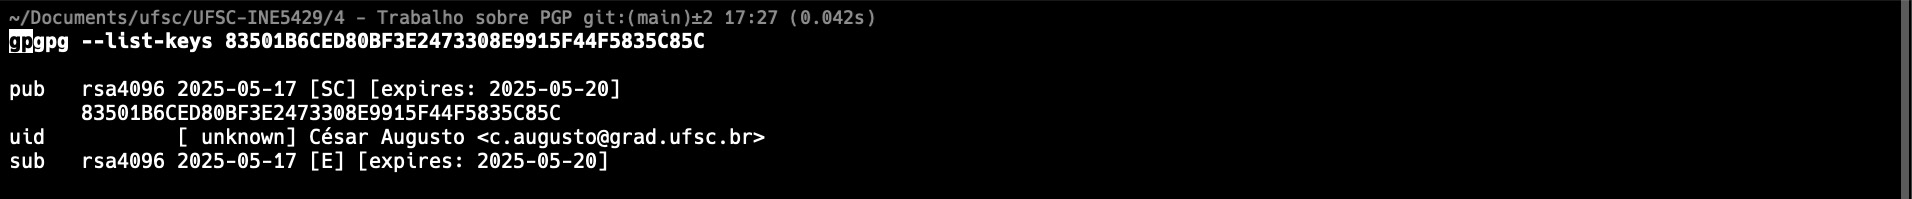
\includegraphics[width=0.8\textwidth]{images/10-verificacao_chave_destinatario.jpg}
    \caption{Verificação da chave do destinatário}
    \label{fig:verificacao-chave-dest}
\end{figure}

\subsubsection{Criptografia do arquivo}
A chave pública do destinatário foi utilizada para criptografar o arquivo, garantindo que apenas ele pudesse decifrá-lo com sua chave privada \cite{rfc4880}:

\begin{lstlisting}[language=bash]
# Criptografia do arquivo usando a chave pública do destinatário
gpg --encrypt --recipient 83501B6CED80BF3E2473308E9915F44F5835C85C --output mensagem_secreta_cesar.txt.gpg mensagem_secreta.txt
\end{lstlisting}

\begin{figure}[htb]
    \centering
    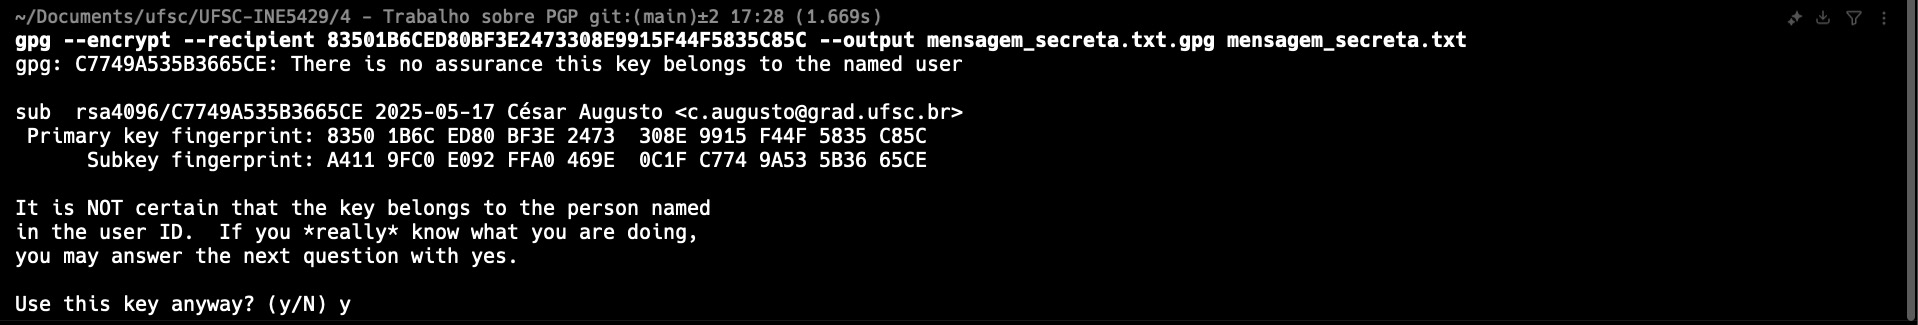
\includegraphics[width=0.8\textwidth]{images/10-criptografia_arquivo.jpg}
    \caption{Criptografia do arquivo}
    \label{fig:criptografia-arquivo}
\end{figure}

\subsubsection{Verificação do arquivo criptografado}
Após a criptografia, o conteúdo do arquivo criptografado foi examinado para confirmar que estava em formato binário e ilegível:

\begin{lstlisting}[language=bash]
# Exibição do conteúdo do arquivo criptografado
hexdump -C mensagem_secreta.txt.gpg | head
\end{lstlisting}

\begin{figure}[htb]
    \centering
    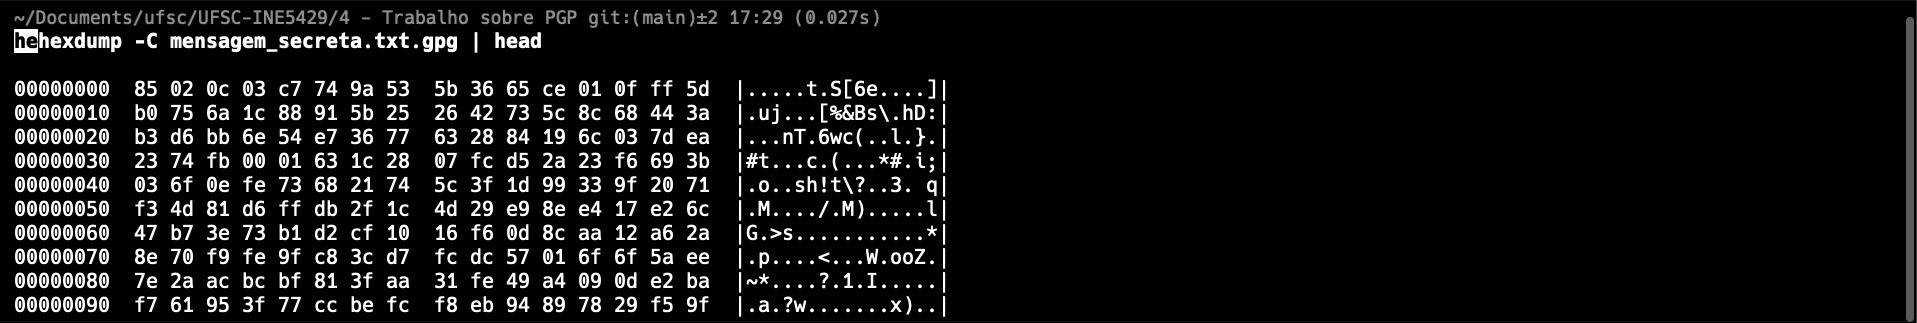
\includegraphics[width=0.8\textwidth]{images/10-verificacao_arquivo_criptografado.jpg}
    \caption{Verificação do arquivo criptografado}
    \label{fig:verificacao-arq-cripto}
\end{figure}

\subsubsection{Envio do arquivo criptografado}
O arquivo criptografado foi enviado para o destinatário via WhatsApp. O arquivo poderia ser enviado por qualquer meio, já que seu conteúdo estava protegido pela criptografia \cite{pgpbest}.

\begin{figure}[htb]
    \centering
    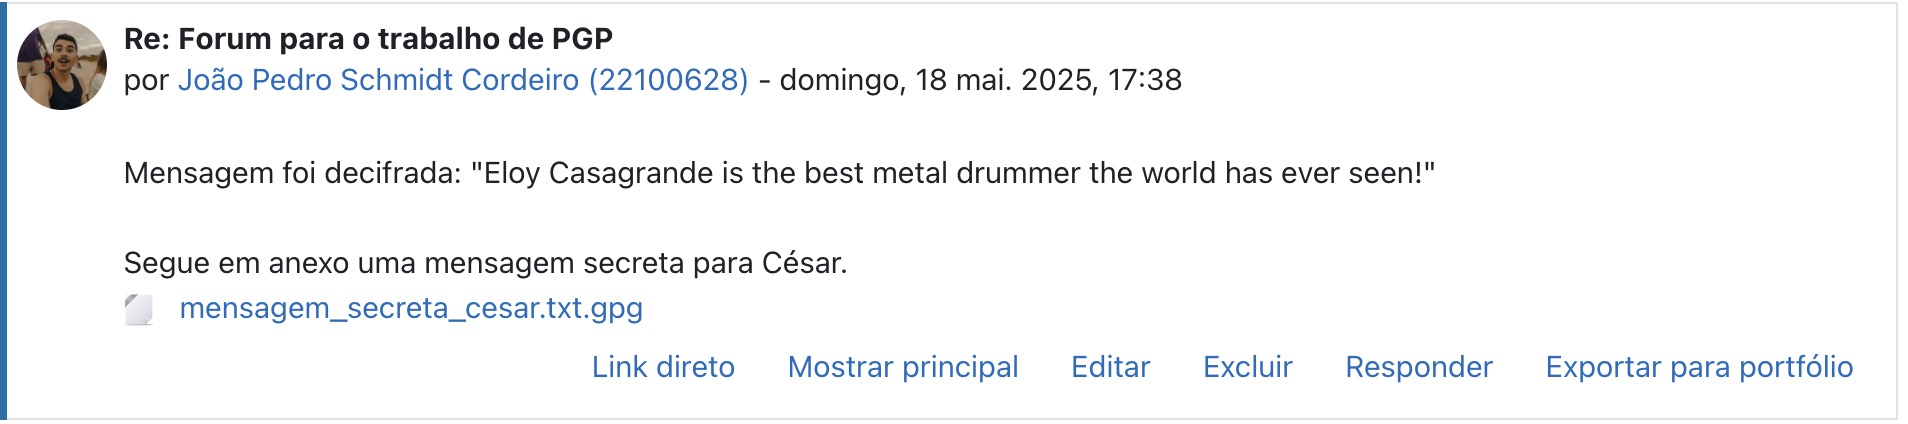
\includegraphics[width=0.8\textwidth]{images/10-envio_arquivo.jpg}
    \caption{Envio do arquivo criptografado}
    \label{fig:envio-arquivo}
\end{figure}

\subsection{Parte 2: Recebendo e decifrando um arquivo sigiloso}

\subsubsection{Recebimento do arquivo criptografado}
Foi recebido do César Augusto um arquivo criptografado chamado \texttt{mensagem\_secreta\_joao.txt.gpg}. Este arquivo havia sido criptografado utilizando a chave pública do autor, de modo que apenas ele poderia decifrá-lo.

\begin{figure}[htb]
    \centering
    
\includegraphics[width=0.8\textwidth]{images/10-recebimento_arquivo.jpg}
    \caption{Recebimento do arquivo criptografado}
    \label{fig:recebimento-arquivo}
\end{figure}

\subsubsection{Decriptação do arquivo}
Para decifrar o arquivo, foi utilizada a chave privada do autor:

\begin{lstlisting}[language=bash]
# Decriptação do arquivo recebido
gpg --decrypt --output mensagem_recebida.txt mensagem_secreta_joao.txt.gpg
\end{lstlisting}

Durante o processo, o sistema solicitou a senha da chave privada para autorizar a decriptação.

\begin{figure}[htb]
    \centering
    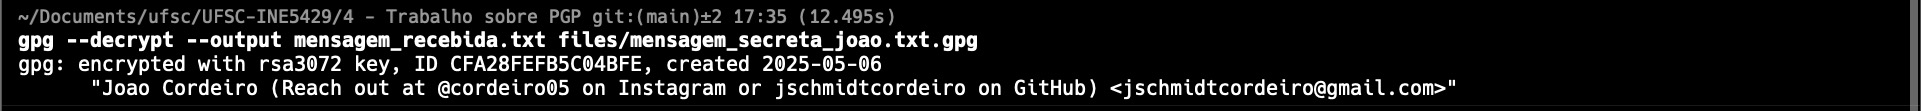
\includegraphics[width=0.8\textwidth]{images/10-decriptacao_arquivo.jpg}
    \caption{Decriptação do arquivo}
    \label{fig:decriptacao-arquivo}
\end{figure}

\subsubsection{Verificação do conteúdo original}
Após a decriptação, o conteúdo original do arquivo pôde ser verificado:

\begin{lstlisting}[language=bash]
# Visualização do conteúdo decifrado
cat mensagem_recebida.txt
\end{lstlisting}

\begin{figure}[htb]
    \centering
    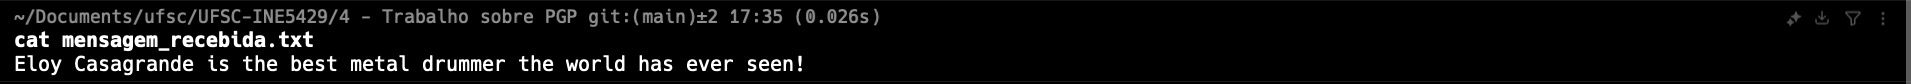
\includegraphics[width=0.8\textwidth]{images/10-conteudo_decifrado.jpg}
    \caption{Conteúdo decifrado}
    \label{fig:conteudo-decifrado}
\end{figure}

\subsection{Resultados e observações}

Este experimento demonstrou com sucesso o processo de proteção de arquivos sensíveis usando criptografia assimétrica PGP. Pontos importantes a serem destacados \cite{gnupgdoc}:

\begin{enumerate}
    \item \textbf{Segurança assimétrica:} Apenas o possuidor da chave privada correspondente pode decifrar um arquivo criptografado com uma chave pública
    \item \textbf{Praticidade:} A criptografia PGP integra-se bem aos fluxos de trabalho existentes
    \item \textbf{Versatilidade:} Qualquer tipo de arquivo pode ser protegido, não apenas mensagens de texto
    \item \textbf{Comunicação segura:} Nenhum meio de comunicação seguro foi necessário para o transporte do arquivo
\end{enumerate}

Estes procedimentos podem ser aplicados a qualquer tipo de arquivo que necessite de confidencialidade, como documentos sensíveis, backups pessoais, ou comunicações privadas. A chave para a segurança do sistema é a proteção adequada da chave privada, que nunca deve ser compartilhada e deve ser protegida por uma senha forte \cite{pgpbest}.

\section{Mostre um exemplo de como assinar um arquivo usando o PGP}

Para demonstrar o processo de assinatura digital utilizando o PGP, foram realizados dois tipos de assinatura em arquivos: uma com assinatura anexada (inline) e outra com assinatura separada (detached). Em seguida, foram trocadas mensagens assinadas com o colega Enzo Nicolas, para validar o processo de verificação de assinaturas \cite{gnupgkeysigning}.

\subsection{Parte 1: Criação de assinaturas digitais}

A assinatura digital serve para garantir a autenticidade e integridade de um arquivo - confirmando que ele foi criado por quem afirma tê-lo criado e que não foi modificado desde então \cite{rfc4880}.

\subsubsection{Preparação dos arquivos para assinar}

Foram criados dois arquivos de texto simples para serem assinados:

\begin{lstlisting}[language=bash]
# Criação do primeiro arquivo para assinatura anexada
echo "Este é um documento importante que precisa ser assinado para comprovar sua autenticidade. Esta assinatura será anexada ao conteúdo original." > files/documento_assinatura_anexada.txt

# Criação do segundo arquivo para assinatura separada
echo "Este é outro documento importante que será assinado digitalmente. Esta assinatura será mantida em um arquivo separado." > files/documento_assinatura_separada.txt
\end{lstlisting}

\subsubsection{Criação de assinatura anexada (inline)}

Neste método, o conteúdo original e a assinatura são combinados em um único arquivo:

\begin{lstlisting}[language=bash]
# Assinatura anexada
gpg --sign --output files/documento_assinado.txt.gpg files/documento_assinatura_anexada.txt
\end{lstlisting}

\begin{figure}[htb]
    \centering
    
\includegraphics[width=0.8\textwidth]{images/11-criacao_assinatura_anexada.jpg}
    \caption{Criação de assinatura anexada}
    \label{fig:criacao-assinatura-anexada}
\end{figure}

O arquivo resultante (\texttt{documento\_assinado.txt.gpg}) contém tanto o conteúdo original quanto a assinatura, mas em formato binário.

\subsubsection{Criação de assinatura separada (detached)}

Neste método, a assinatura é armazenada em um arquivo separado, mantendo o arquivo original intacto:

\begin{lstlisting}[language=bash]
# Assinatura separada
gpg --detach-sign files/documento_assinatura_separada.txt
\end{lstlisting}

\begin{figure}[htb]
    \centering
    
\includegraphics[width=0.8\textwidth]{images/11-criacao_assinatura_separada.jpg}
    \caption{Criação de assinatura separada}
    \label{fig:criacao-assinatura-separada}
\end{figure}

O comando gera um arquivo de assinatura chamado \texttt{documento\_assinatura\_separada.txt.sig}, enquanto o arquivo original permanece inalterado.

\subsubsection{Verificação local das assinaturas}

Antes de enviar as assinaturas, foram verificadas localmente se estavam funcionando corretamente:

\begin{lstlisting}[language=bash]
# Verificação da assinatura anexada
gpg --decrypt files/documento_assinado.txt.gpg

# Verificação da assinatura separada
gpg --verify files/documento_assinatura_separada.txt.sig files/documento_assinatura_separada.txt
\end{lstlisting}

\begin{figure}[htb]
    \centering
    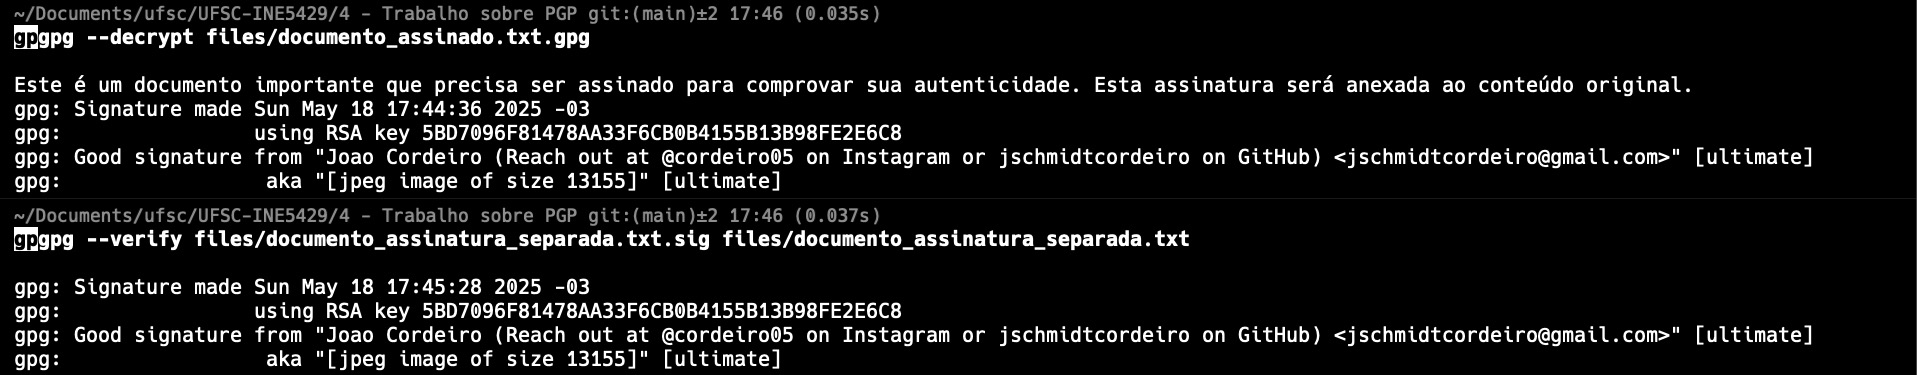
\includegraphics[width=0.8\textwidth]{images/11-verificacao_local_assinaturas.jpg}
    \caption{Verificação local das assinaturas}
    \label{fig:verificacao-local-assinaturas}
\end{figure}

\subsection{Parte 2: Troca de arquivos assinados com um colega}

\subsubsection{Envio dos arquivos assinados}

Foram enviados para o César Augusto os seguintes arquivos:
\begin{itemize}
    \item Para a assinatura anexada: apenas o arquivo \texttt{documento\_assinado.txt.gpg}
    \item Para a assinatura separada: tanto o arquivo original \texttt{documento\_assinatura\_separada.txt} quanto a assinatura \texttt{documento\_assinatura\_separada.txt.sig}
\end{itemize}

\begin{lstlisting}[language=bash]
# Compactação dos arquivos para envio
zip files/arquivos_assinados.zip files/documento_assinado.txt.gpg files/documento_assinatura_separada.txt files/documento_assinatura_separada.txt.sig
\end{lstlisting}

\begin{figure}[htb]
    \centering
    
\includegraphics[width=0.8\textwidth]{images/11-envio_arquivos_assinados.jpg}
    \caption{Envio dos arquivos assinados}
    \label{fig:envio-arquivos-assinados}
\end{figure}

\subsubsection{Recebimento de arquivos assinados}

Foram recebidos do César Augusto os arquivos correspondentes:
\begin{itemize}
    \item Um arquivo com assinatura anexada: \texttt{files/arquivo\_assinado.txt.gpg}
    \item Um arquivo original e sua assinatura separada: \texttt{files/arquivo\_assinado.txt} e \texttt{files/arquivo\_assinado.txt.sig}
\end{itemize}

\begin{figure}[htb]
    \centering
    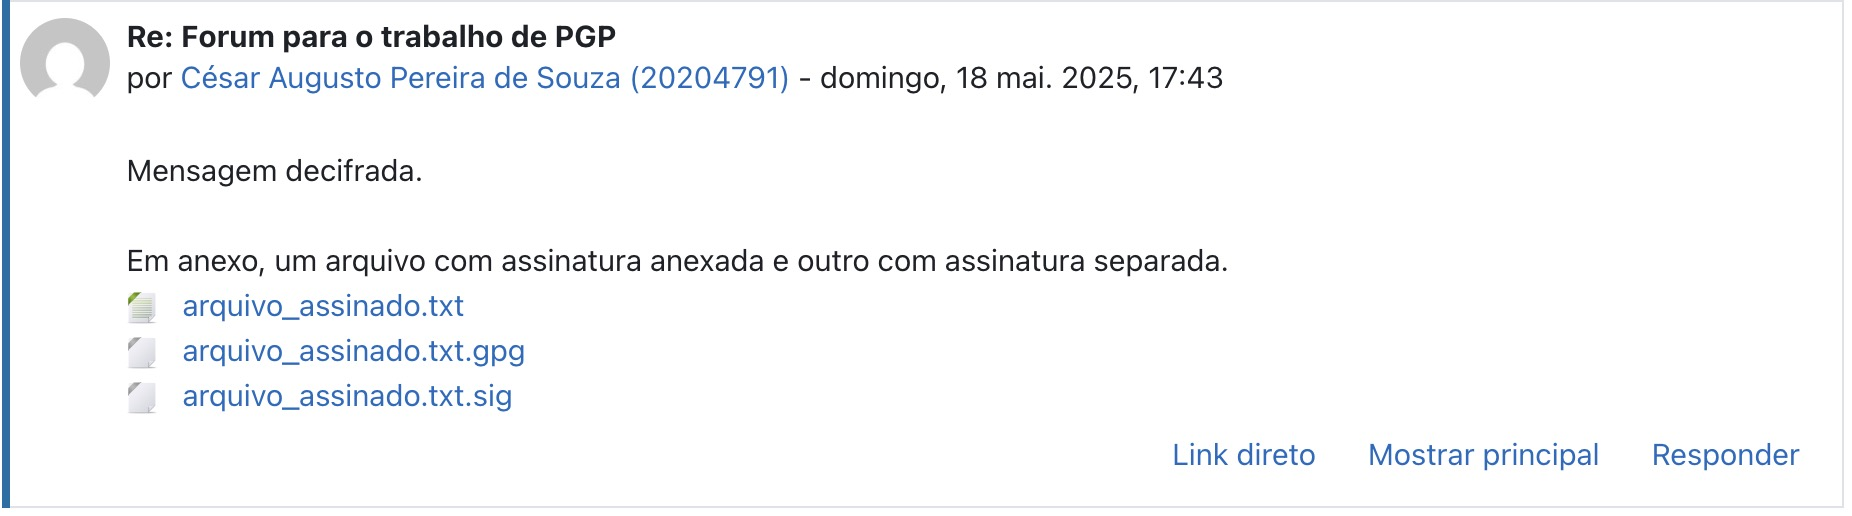
\includegraphics[width=0.8\textwidth]{images/11-recebimento_arquivos_assinados.jpg}
    \caption{Recebimento dos arquivos assinados}
    \label{fig:recebimento-arquivos-assinados}
\end{figure}

\subsection{Parte 3: Verificação das assinaturas recebidas}

\subsubsection{Verificação da assinatura anexada}

Para verificar a assinatura anexada, foi utilizado o comando de decriptação do GPG, que também verifica a assinatura:

\begin{lstlisting}[language=bash]
# Verificação da assinatura anexada e extração do conteúdo
gpg --decrypt files/arquivo_assinado.txt.gpg > files/arquivo_anexado_conteudo.txt
\end{lstlisting}

\begin{figure}[htb]
    \centering
    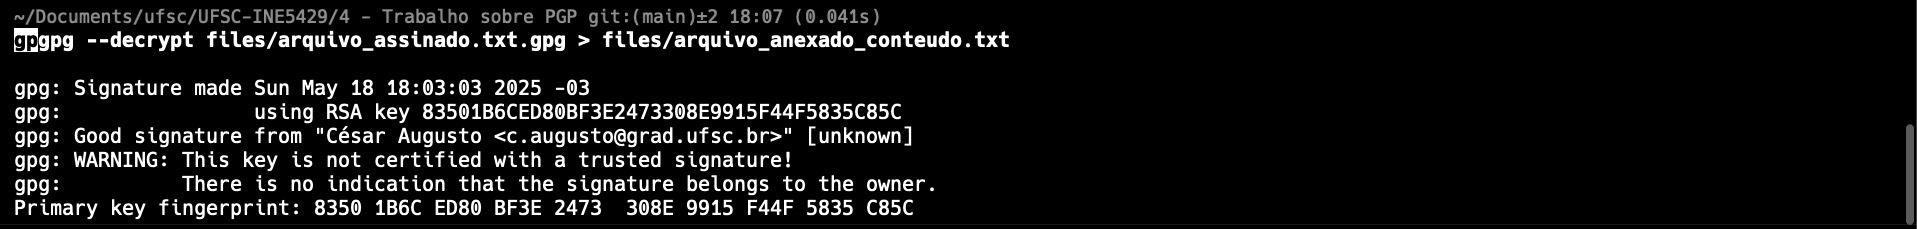
\includegraphics[width=0.8\textwidth]{images/11-verificacao_assinatura_anexada.jpg}
    \caption{Verificação da assinatura anexada}
    \label{fig:verificacao-assinatura-anexada}
\end{figure}

\subsubsection{Verificação da assinatura separada}

Para a assinatura separada, foi utilizado o comando específico de verificação:

\begin{lstlisting}[language=bash]
# Verificação da assinatura separada
gpg --verify files/arquivo_assinado.txt.sig files/arquivo_assinado.txt
\end{lstlisting}

\begin{figure}[htb]
    \centering
    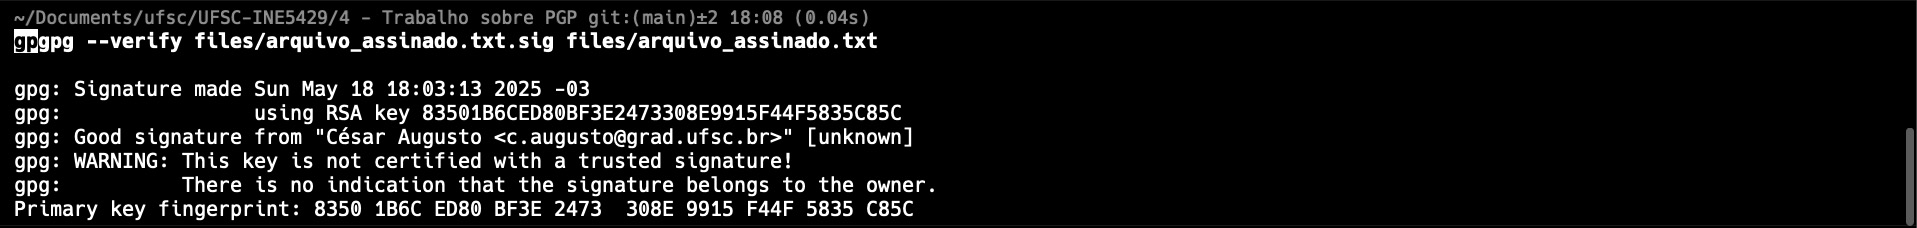
\includegraphics[width=0.8\textwidth]{images/11-verificacao_assinatura_separada.jpg}
    \caption{Verificação da assinatura separada}
    \label{fig:verificacao-assinatura-separada}
\end{figure}

\subsubsection{Inspeção do conteúdo das mensagens}

Após confirmar a autenticidade das assinaturas, foi possível visualizar o conteúdo das mensagens com segurança:

\begin{lstlisting}[language=bash]
# Visualização do conteúdo da mensagem com assinatura anexada
cat files/arquivo_anexado_conteudo.txt

# Visualização do conteúdo da mensagem com assinatura separada
cat files/arquivo_assinado.txt
\end{lstlisting}

\begin{figure}[htb]
    \centering
    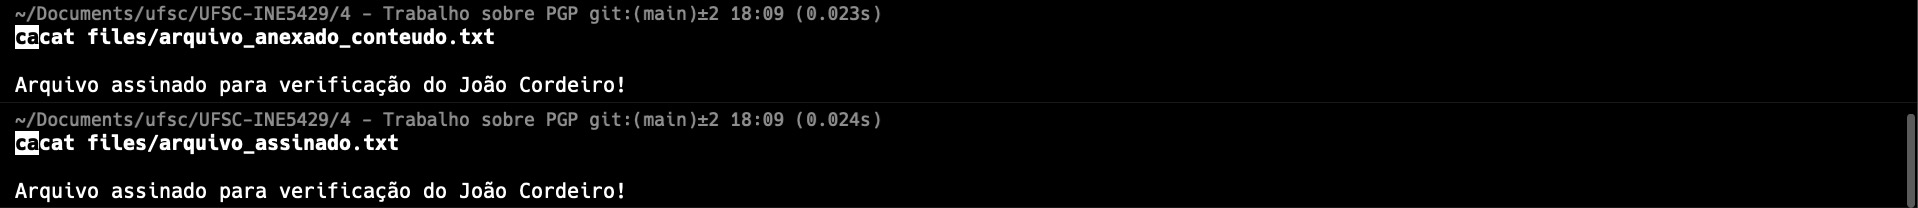
\includegraphics[width=0.8\textwidth]{images/11-conteudo_mensagens_verificadas.jpg}
    \caption{Conteúdo das mensagens verificadas}
    \label{fig:conteudo-mensagens-verificadas}
\end{figure}

\subsection{Resultados e observações}

Este experimento demonstrou com sucesso o processo de assinatura digital e verificação utilizando o PGP \cite{gnupgkeysigning}. Pontos importantes:

\begin{enumerate}
    \item \textbf{Integridade garantida:} Qualquer alteração no conteúdo original invalidaria a assinatura
    \item \textbf{Autenticidade confirmada:} A verificação bem-sucedida comprova que o arquivo foi realmente assinado pelo remetente
    \item \textbf{Diferenças entre os métodos:}
    \begin{itemize}
        \item \textbf{Assinatura anexada:} Conveniente por manter tudo em um arquivo, mas modifica o formato original
        \item \textbf{Assinatura separada:} Mantém o arquivo original intacto, ideal para documentos que não devem ser modificados
    \end{itemize}
\end{enumerate}

Ambos os métodos são eficazes para garantir a autenticidade e integridade das comunicações digitais. A escolha entre eles depende dos requisitos específicos de cada situação \cite{pgpbest}.